Now that the light potentials have been measured, we elaborate in this chapter how it was implemented in an real-world experiment on ultra-cold atoms, initially using Rb atoms.
In order to do this, a new setup was constructed.
The construction of the vacuum and atom source part can be found in \cref{sec:VacuumAtom}.
The laser system is explained in \cref{sec:LaserSystem}.
Images of the MOT are displayed in \cref{sec:MOTresult}.
We finish up with how overlap this MOT with our tweezer array (\cref{sec:Tweezers}) and how to image the tweezers (\cref{sec:TweezerImaging}).

\section{Vacuum and Atom Source}\label{sec:VacuumAtom}

The vacuum and atom source of the setup was designed with compactness in mind. 
The core of the experiment is the glass cell (30 mm outer and 4.0 mm wall thickness, optically contacted)\footnote{The glass cell was provided to us by our collaborators from the University of Amsterdam.}.
The glass cell can be seen in a CAD drawing and in real life in \cref{fig:VacuumSetup,fig:Chamber}.
It is pumped down to the ultra-high vacuum regime, which is need to minimize collisions with the background gas and improve the lifetime of the atoms in the tweezers.
To pump the cell down, the glass cell is connected to a vacuum chamber (\cref{fig:VacuumSetup}, left).
To allow for more room around the glass cell, in between the vacuum vessel and the glass cell an extension tube is added.
We attach a turbomolecular pump to the chamber using a valve (not shown in the figure) and pump down to $\sim 10^{8}$ mbar.
This pressure was measured using a pressure Gauge (\cref{fig:Chamber}).
To reach a better vacuum, the system was baked for a duration of two weeks at 130${}^{\circ}$C by Rik van Herk \cite{Herk2022}.

As atom source, a triplet of Rb dispensers\footnote{SAES Getters Alkali Metal Dispensers.} is used.
The amount of Rb released can be controlled by the current running through the dispensers.
We typically run the dispensers at $\sim$ 5A.
The dispensers are mounted to the vacuum chamber using a CF40 adapter made by Eddy Rietman.
We first ran the dispensers for 30 minutes while leaving the turbo pump on to get rid of the oxidation layer on the dispenser.
This lead to a brief but significant increase in pressure, while we say no atomic fluorescence from Rb in the chamber.  

Next, we activate the non-evaporative getter\footnote{NEXTorr Z 100 NEG - ion combination pump.} by heating it to 500${}^{\circ}$C while pumping away its out gassing using the turbo pump. Finally, after closing the turbo valve and turning on the ion pump we reached a pressure of $\sim 2\times 10^{-10}$ mbar, as measured using the ion pump (the pressure gauge is not designed for pressures this low).
When turning on the dispensers, the pressure briefly spikes to the $10^{-9}$ region but quickly returns back to the $10^{-10}$ regime.

One note: if this Rb machine is to be used for a longer time in the future, it would probably be wise to add a valve between the dispensers and the vacuum vessel, which allows for replacement of the dispensers without venting the entire chamber. 





\begin{figure}
	\begin{subfigure}{.54\linewidth}
		\centering
		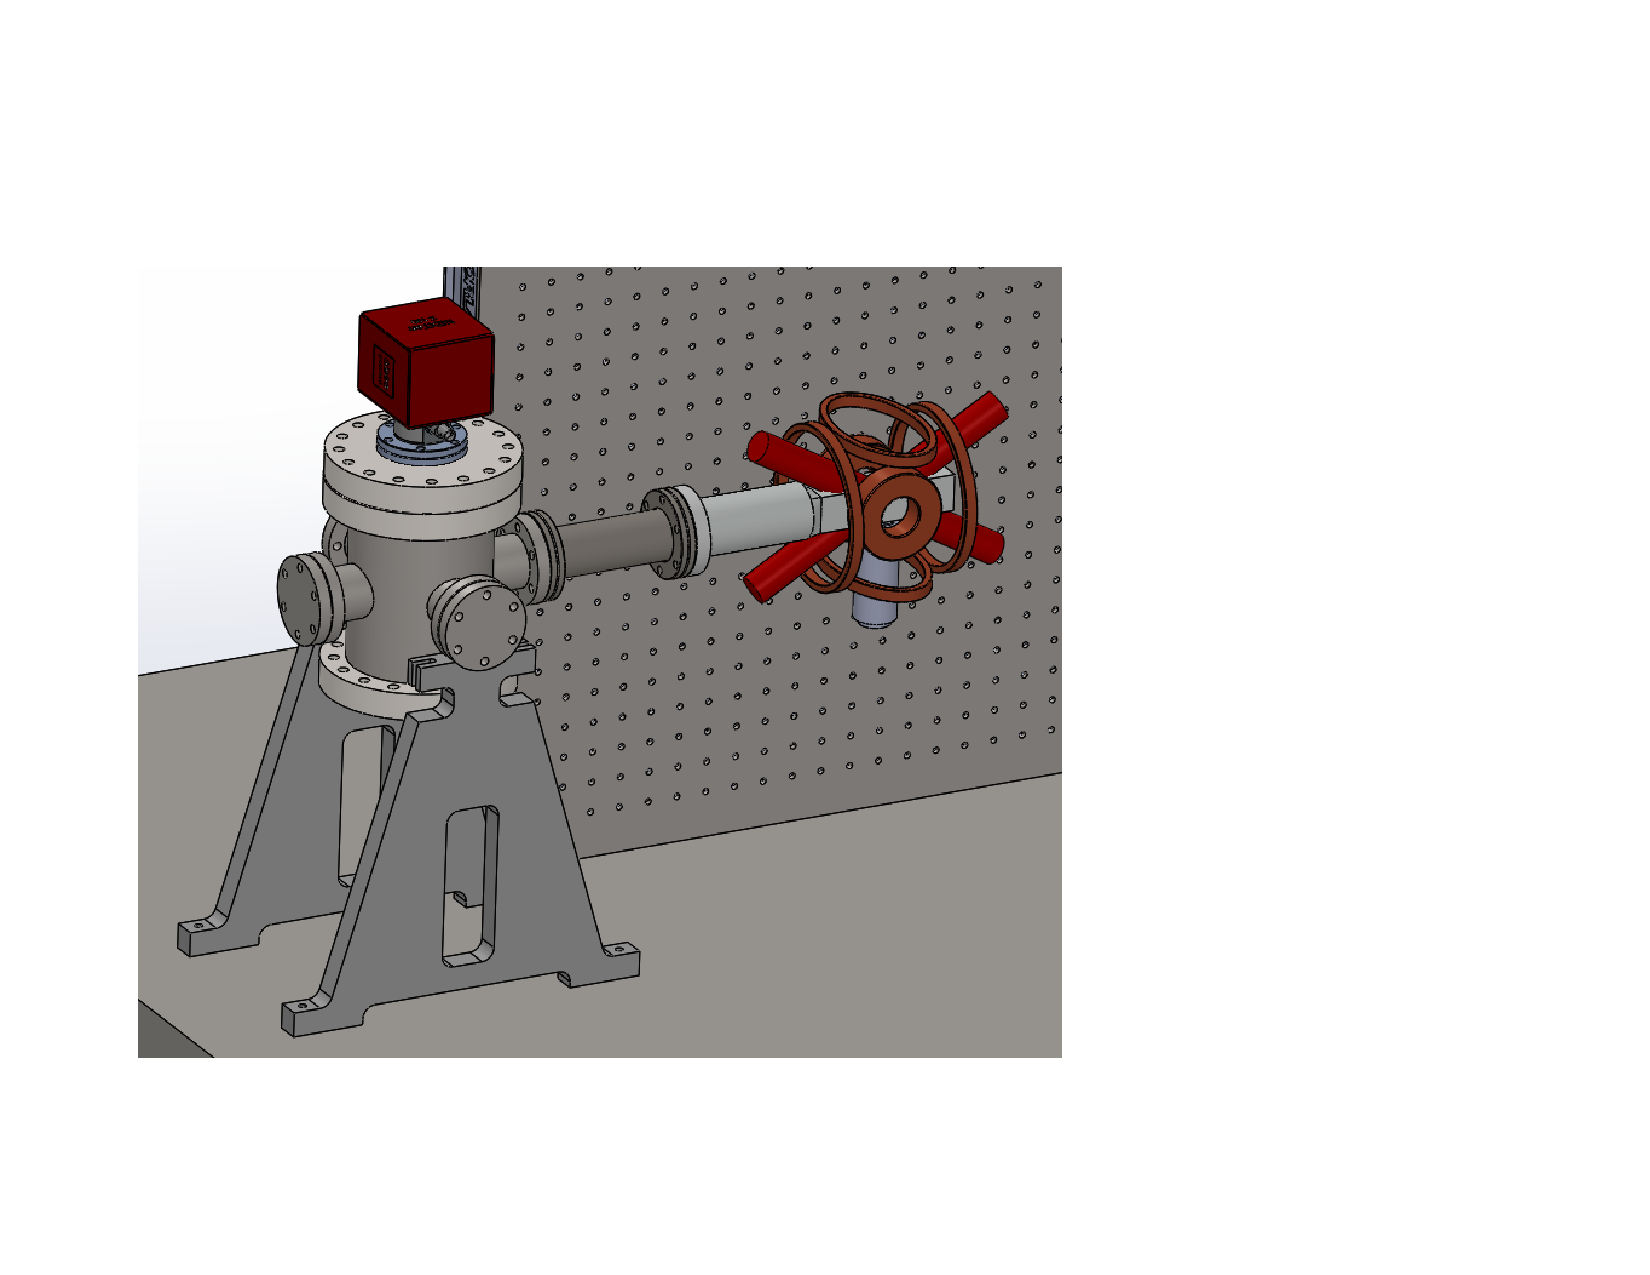
\includegraphics[height=6cm]{figures/Vacuum.pdf}
		\caption{}
		\label{fig:VacuumSetup}
	\end{subfigure}
	\hfill
	\begin{subfigure}{.44\linewidth}
		\centering
		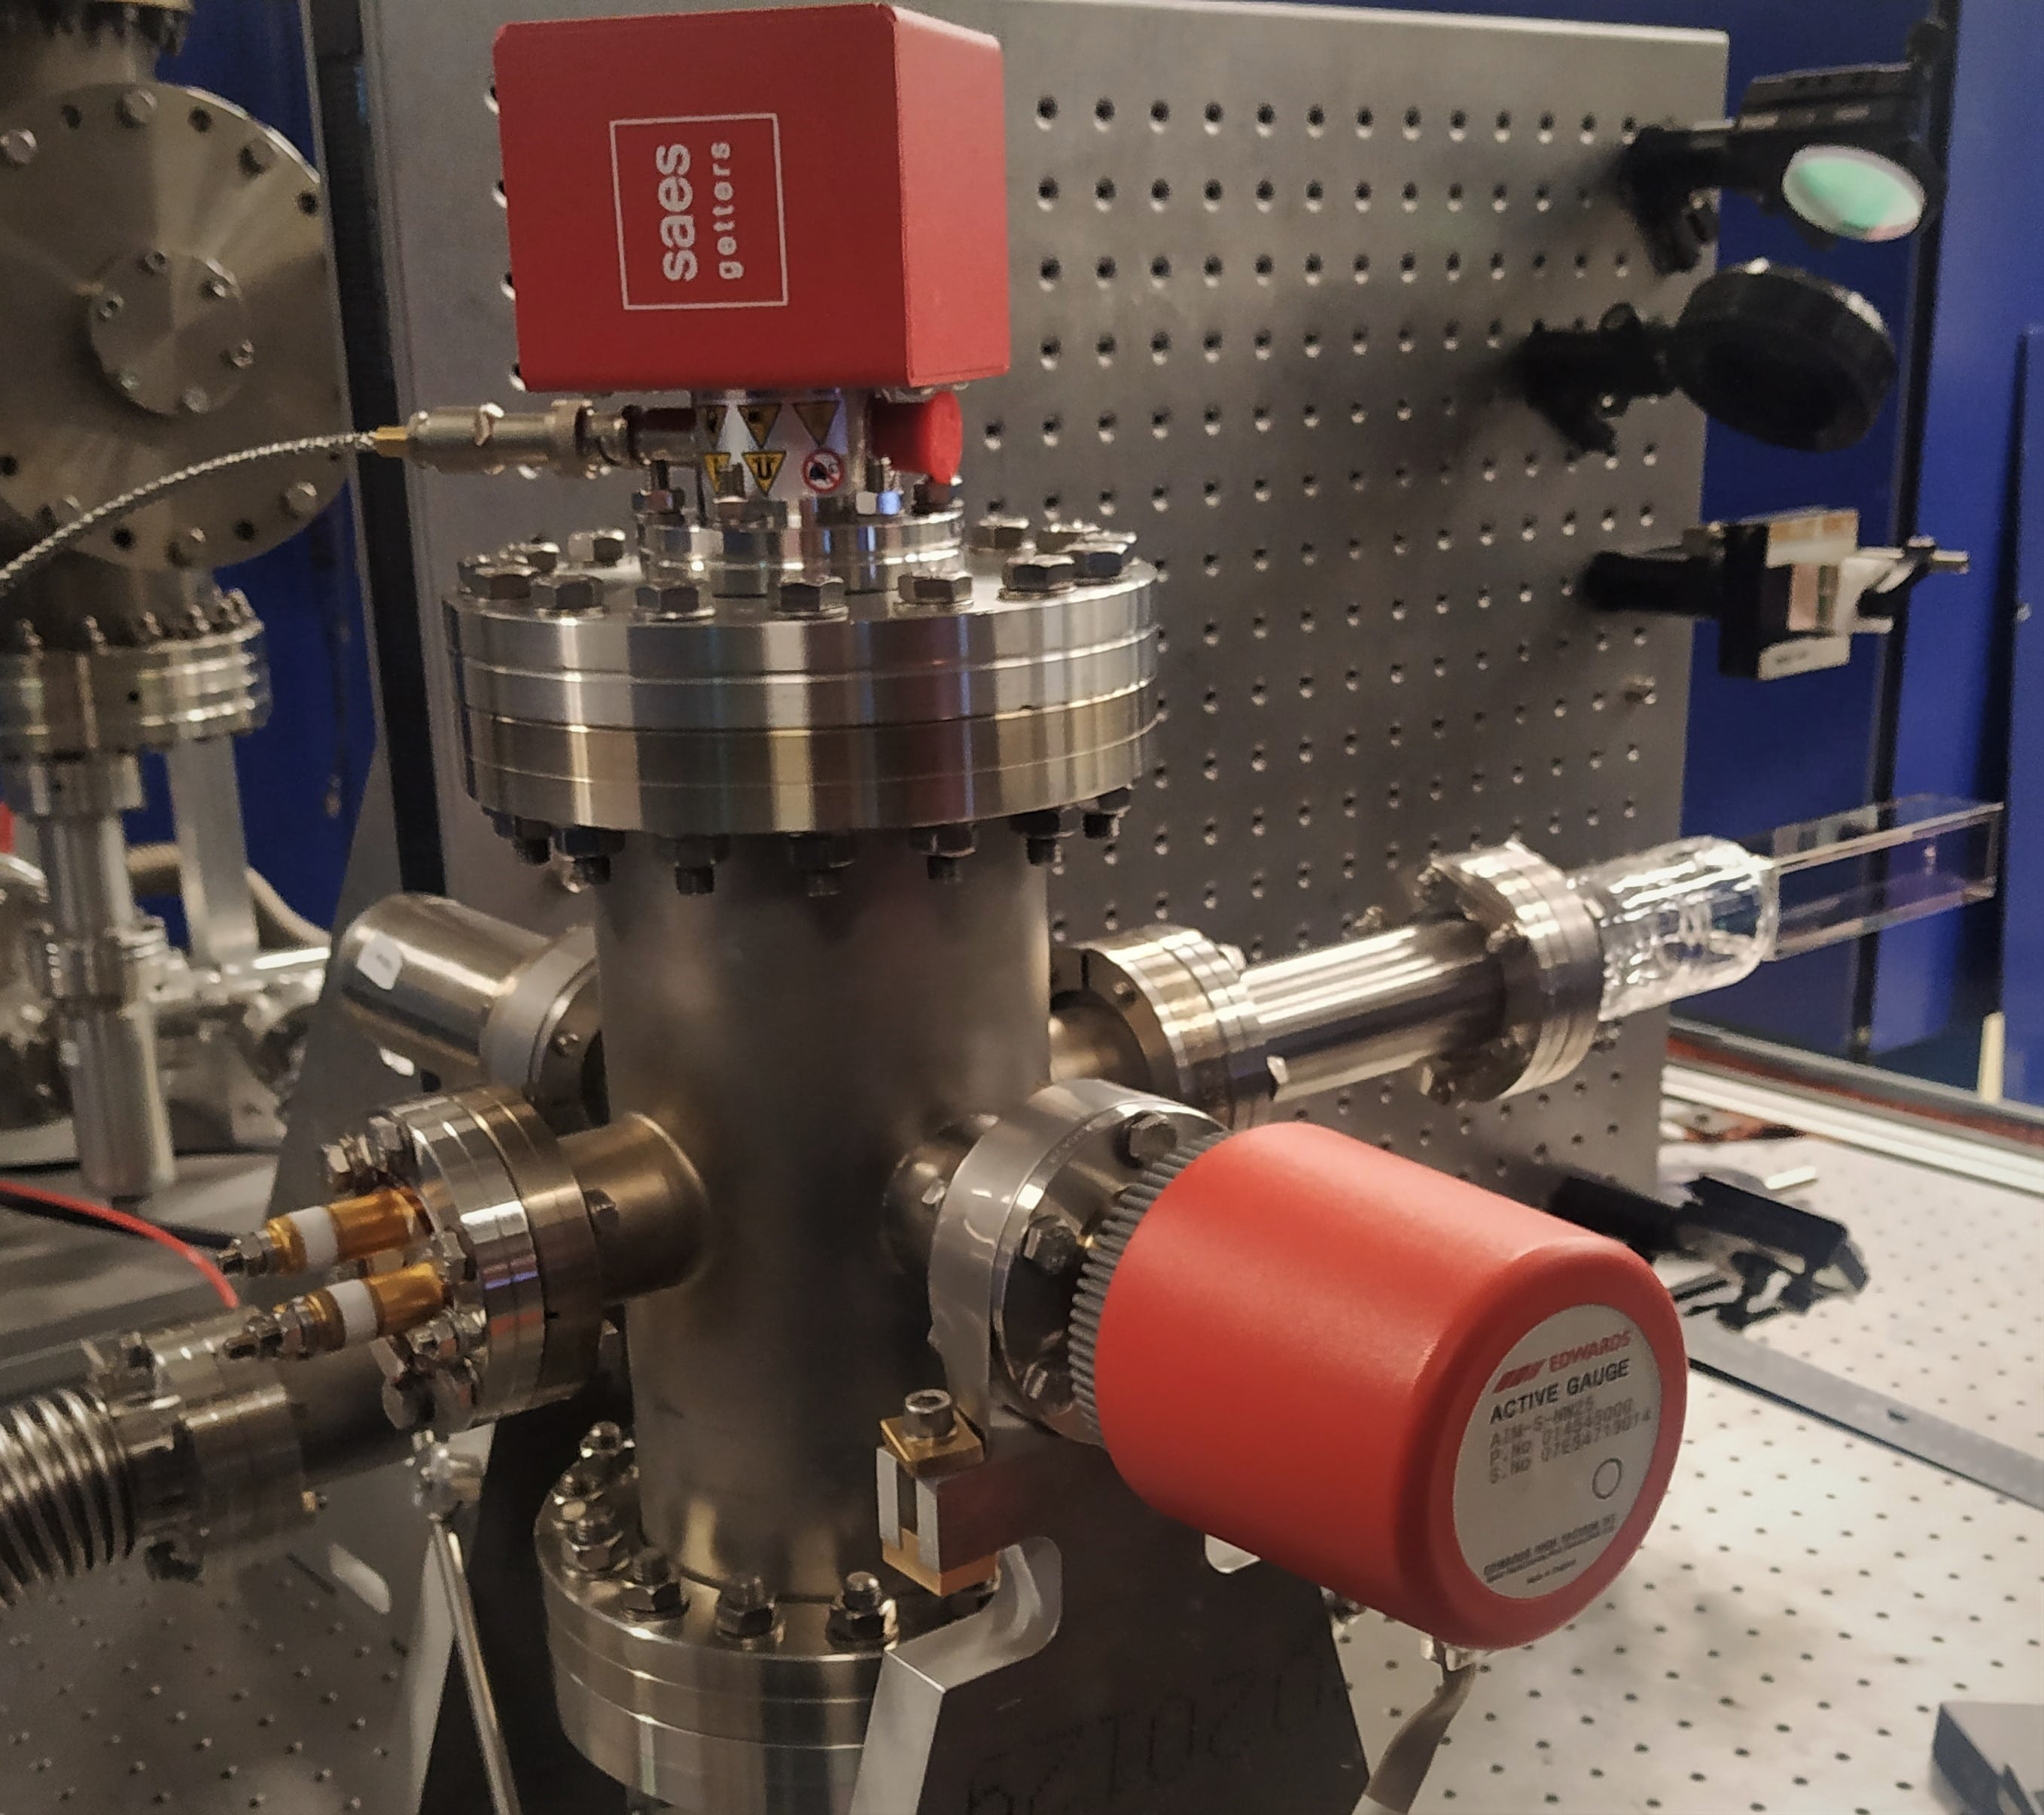
\includegraphics[height=6cm]{figures/Chamber.jpg}
		\caption{}
		\label{fig:Chamber}
	\end{subfigure}
	\caption{\textbf{a)} CAD drawing of the vacuum vessel connected to the glass cell on the right. 
	Around the glass cell, 4 out of 6 MOT beams are shown along with the magnetic field coils and a single microscope objective on the bottom. 
	CAD drawing by Eddy Rietman.
	\textbf{b)} Picture of the vacuum components: top: ion/getter pump. Right: glass cell. Also connected to the chamber rom left to right: valve for turbo pump, triplet of Rb dispensers and pressure gauge.}
\end{figure}

\section{Laser System}\label{sec:LaserSystem}

For the laser system we recycled a significant part of the previous setup \cite{Reijnders2010}.
The atomic species we selected is Rb-85 because it is the most abundant isotope. 
a Rb-85 MOT requires two lasers: one to cool and trap the atoms and one to recycle back atoms that end up in the wrong ground state (\cref{sec:PracticeRb}.

\subsection{Cooling/Trapping}

For the laser cooling and trapping beams we used the Toptica DLX110.
This laser should be able to produce $\sim 1$ W of power, but in current condition we typically output $\sim 500$ mW, which is already plenty of power for what we need. 
The repump light is produced by applying sidebands of fixed frequency spacing on the main trapping laser, more on this later.

The laser is shown in \cref{fig:RbLaserSetup}.
After passing an optical isolator, a fraction of laser power is split off to the modulation transfer spectroscopy section after being offset-locked using the lock \ac{AOM} (right) set to $2\pi \times  84.5$ MHz\footnote{From now on, all frequencies are assumed to be angular and we omit the $2\pi$ term.}
Modulation transfer spectroscopy is described elsewhere \cite{McCarron2008,Reijnders2010}, but very briefly: the working principle is that by scanning the probe pulse using the \ac{EOM}, the absorption peak of $D_2$ is found using the Rb cell, which the laser is locked to.  
Contrary, the MOT AOM (top) is set to 80 MHz, which is $2 \times (80 - 84.5) = -9$ MHz from the resonance frequency, which is roughly equivalent to a detuning of $\delta = -1.5 \gamma$.
After passing through the AOMs, the lasers are directed further to the glass cell. 
This is shown in 

\begin{figure}
    \centering
    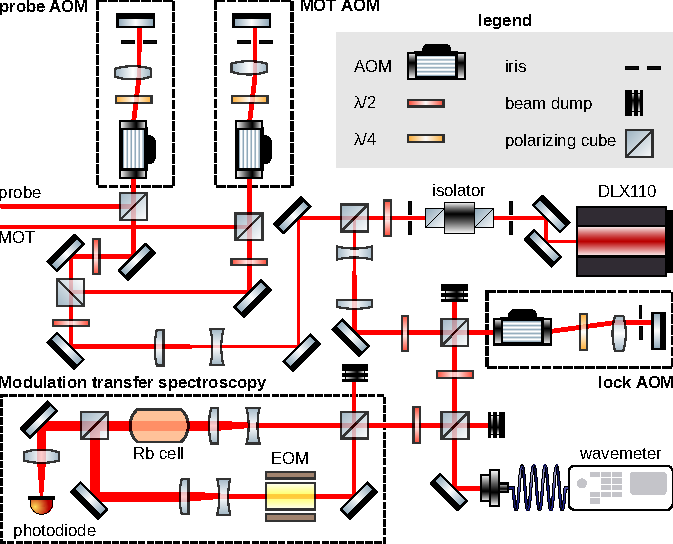
\includegraphics[width=\linewidth]{figures/RbLaserSetup.pdf}
    \caption{Laser system for the trapping and repump laser system for \textsuperscript{85}Rb.
    The bulk was built by \cite{Reijnders2010}.
    A section of laser light is split off to the modulation transfer spectroscopy (bottom left), after first double passing the lock \ac{AOM} (right). 
    Top: set of AOMs for the MOT and probe light.
    All beam splitter cubes shown are polarizing.
    }
    \label{fig:RbLaserSetup}
\end{figure}

\subsection{Repump}

Contrary to the previous setup, we do not use a separate repump laser. 
Instead, we used an \ac{EOM}.
The principle at play here is the electro-optic effect that can be used to modulate a beam of light. 
We drive the EOM with a modulation amplitude $\epsilon$ and frequency $\Omega$.
If the laser beam is described by amplitude $A$ and frequency 'carrier' frequency $\omega = \omega$ as $A = A_0 e^{i \omega_c t}$, after passing through an EOM the amplitude can be described as

\begin{equation}
    A(t) = A_0 e^{i \omega t}(1+i \epsilon \sin(\Omega t)
\end{equation}
where we assumed $\epsilon < 0$. In this case ($\epsilon <0$), most of the power is still contained in the carrier frequency component $\omega_c$, but a small fraction of power is contained in two first-order sidebands at $\omega_c \pm \Omega$.
We can use one of the sidebands as our repump laser. 
The other sideband is unused. 
Now turning our attention to how this was implemented.
The EOM\footnote{7Qubig EO-Rb85-3K} was fed a $\Omega = 2915$ MHz signal provided by a harmonic synthesizer RF\footnote{DS instruments SG6000PRO} providing a signal of $-6.9$dbm.
This signal was amplified by a 45 dB amplifier\footnote{Minicircuits ZHL-16W-43+} which should provide some $\sim 10$\% of power in the first sidebands \cite{Rens2014}, which should be a sufficient amount of power for a repump laser. 
We did not measure the exact fraction of power in the sidebands because we do not have a sufficiently high-finesse wavemeter available, but the current parameters seemed to work satisfactory. 


\section{Characterizing the MOT}\label{sec:MOTresult}

To image the MOT, we have two CCD cameras\footnote{UEye UI-2230SE}.
Both are positioned on a set of translation stages to allow for $X-Y-Z$ translation and are covered by a 780 band-pass filter which is the wavelength of the laser induced fluorescence.
The first camera is positioned above the MOT and is also brought in focus with the tweezer beams. 
The MOT is imaged onto this camera using a $f=50$ mm lens positioned 110 mm from the MOT and 91 mm from the CCD for a magnification of $\sim 0.83$.
The horizontal camera has a larger field of view, which makes it easier to initially find the MOT. 
This camera has a magnification of $0.5$ and has a $f=100$ mm lens. 
   
We estimate the number of captured atoms in the MOT by counting the number of counts on our side camera, subtracting background counts by turning off the field by summing over all pixels in a region of interest around the MOT $\sum_j p_j$.
We keep in mind the exposure time $\tau_s$, which varied but was typically $10$ ms, camera gain $G = 1$ and sensitivity $C$.
The camera sensitivity constant $C$ for this particular camera was determined to be $6 \cdot 10^3$ counts per photon and was calibrated using a variety of ND filters and a laser at 780 nm of known intensity. The total number of atoms is now
 
 \begin{equation}\label{eq:AtomNumber}
     N = \left( \frac{2}{\gamma\beta}\right)
     \left(\frac{4\pi l^2}{R^2}\right)
     \sum_j \frac{p_j}{\tau_s G C}.
 \end{equation}
In \cref{eq:AtomNumber} $\gamma = 2\pi \cdot 6.0 \cdot 10^6$ is the aforementioned linewidth of the D2 transition of Rb-85, $\beta \sim 0.6$ is a parameter taking into account photon loss of the glass cell and band-pass filter, $l = 20$ cm is the distance from the MOT to the collection lens and $R = 25$ mm is its radius. 
We typically find a an atom number $\sim 10^5$.
This is a relatively small number of atoms, but still orders of magnitude more than we need for loading them in arrays of optical tweezers. 
A possible explanation for the rather small number of atoms is that the unbalance in the various MOT beams: as a result of the rather large angle the vertical MOT beams make with the glass cell to make room for the microscope objective(s), there is significant loss of power in the retro-reflected beam, which has to pass the glass cell twice. 
In a next iteration of this Rb machine or a Sr equivalent, it would be useful to have 6 independent laser beams instead of 3 retro-reflected ones, though this comes at a cost of requiring more power. 
But the quantity that is of more relevance for optical tweezers is the MOT temperature, which was measured by Rik van Herk to be $200$ $\mu$K \cite{Herk2022}, which is slightly above the Doppler temperature. 
 
 


\section{Tweezer Arrays}\label{sec:Tweezers}

\begin{figure}
    \centering
    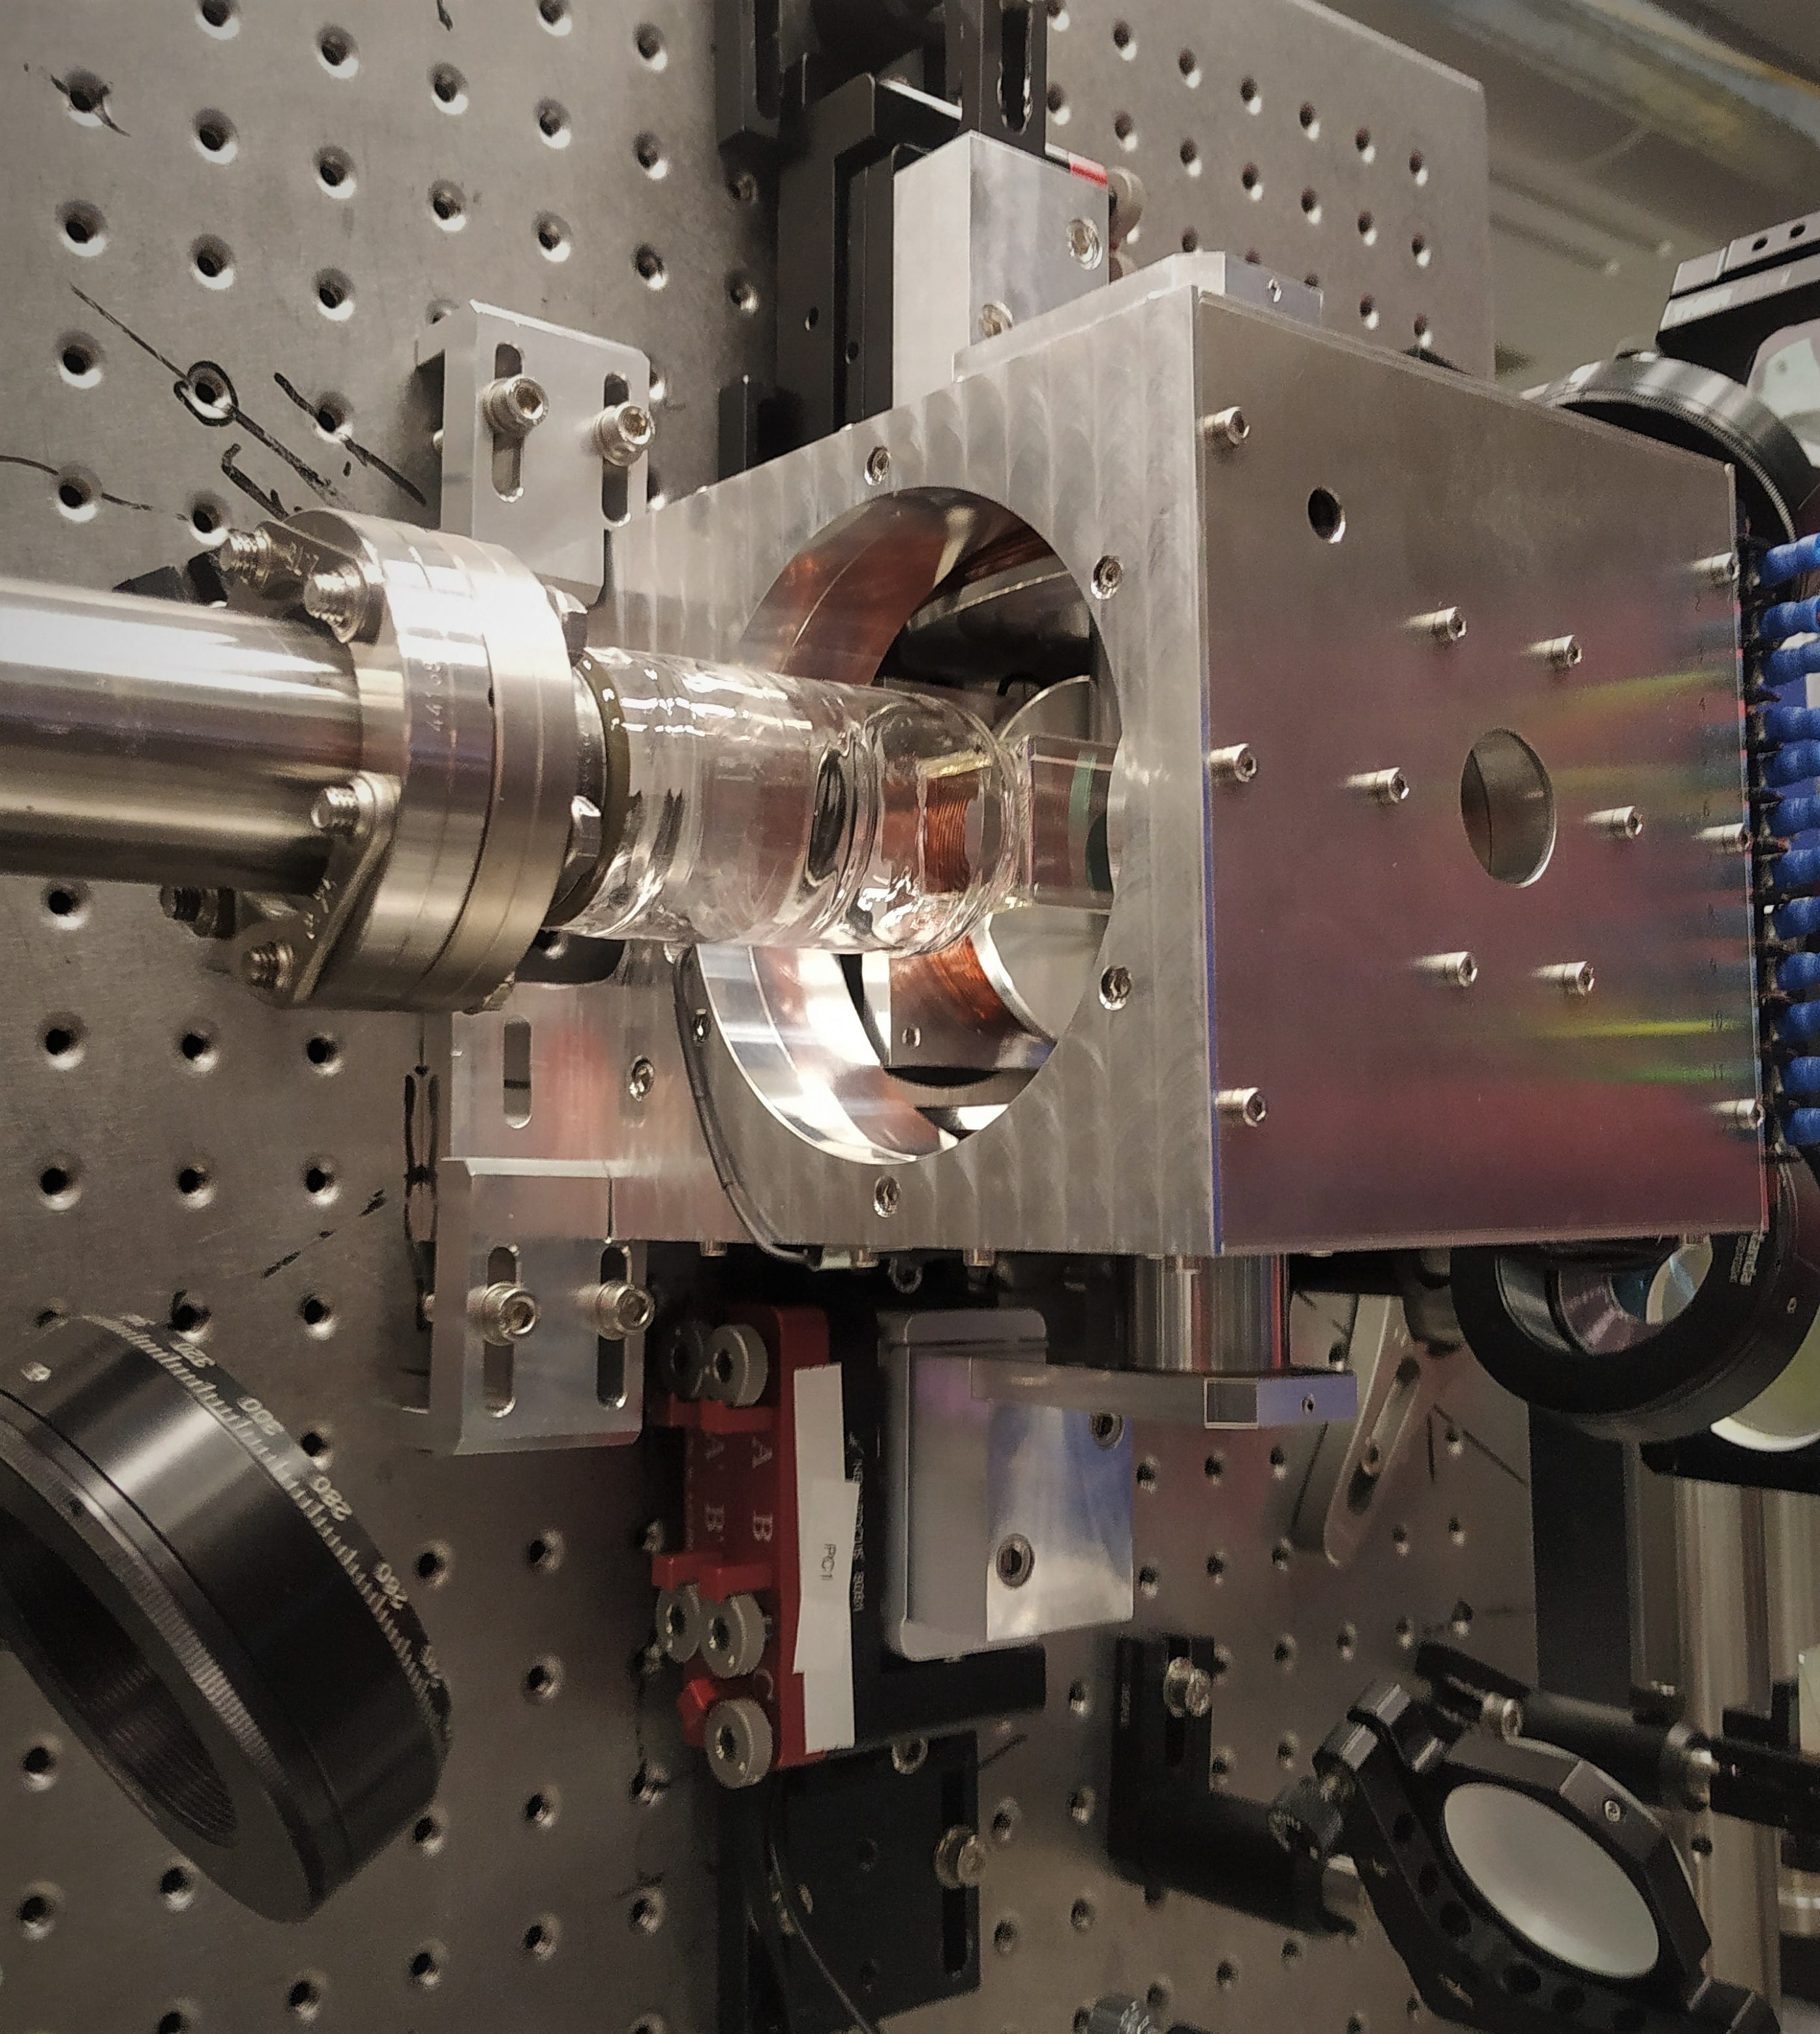
\includegraphics[width=0.5\textwidth]{figures/Coils.jpg}
    \caption{Housing for the magnetic field coils, as well as a microscope on a 5-axis stage on bottom and top. 
    For placement on arbitrary locations on the breadboard, the stages are not directly fixed in the table but in a set of base plates. 
    The microscope objective is mounted on the stage using a custom holder.}
    \label{fig:Coils}
\end{figure}



\subsection{Overlapping the MOT with the tweezer}

\begin{itemize}
    \item Top camera: get focus more or less right with 50 mm lens, as well as align tweezer
    \item Scan tweezer over resonance, try to see off balance of MOT from side camera. 
\end{itemize}

\section{Imaging Tweezer Arrays}\label{sec:TweezerImaging}

The collection angle $\eta$ is $2\pi(1-cos{\alpha})/4\pi$ where $\alpha$ is the maximum angle from the optical axis of the imaging system. $\alpha=\arcsin{0.5}$ the collection angle is $\eta = 0.067$

\begin{figure}
    \centering
    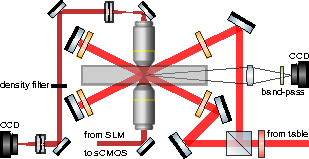
\includegraphics[width=\textwidth]{figures/MOTsideview.pdf}
    \caption{Caption}
    \label{fig:my_label}
\end{figure}

\begin{figure}
    \centering
    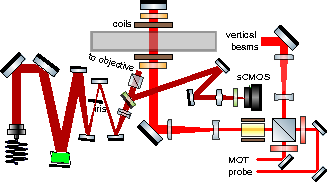
\includegraphics[width=0.6\textwidth]{figures/MOTupview.pdf}
    \caption{Caption}
    \label{fig:my_label}
\end{figure}


